%% introduction.tex
%%

%% ==============================
\chapter{Introduction}
\label{ch:Introduction}
%% ==============================
	Ever since the beginning of the \nth{19} century science in general but especially the field of physics has been undergoing an unbelievably quick and vast development. The possibilities arising from automated analysis through the use of advanced computation grids connected to the optimization of manufacturing processes for detectors leave the world - and even scientists - amazed. Nevertheless, with more and more phenomena well understood, the remaining tasks often require huge projects and large collaborations. One of these projects, aimed to determine the effective mass of the electron anti-neutrino, is the KATRIN experiment.
	Working on the project is a liaison of 15 universities and research facilities with over 150 coworkers aspiring to find the absolute neutrino mass scale.\\
	This chapter will put the KATRIN experiment in the context of neutrino physics in general. At first, an introduction covering the postulation and discovery of the neutrino is given (section 1.1), followed by a discussion on different neutrino sources (section \ref{ch:Introduction:sec:neutrinoSources}) and the role of neutrinos in the Standard Model (section \ref{ch:Introduction:sec:Neutrinos in the Standard Model}) as well as latest results from research, most notably neutrino oscillations (section \ref{ch:Introduction:sec:neutrino Oscillations}). The different methods to determine the neutrino mass scale are illustrated in sections 1.5 and 1.6.
	Finally, section \ref{ch:Introduction:sec:Cosmic Air Showers} will be devoted to cosmic air showers, which are of importance in the context of this thesis.
	
	\section{Neutrinos - the early years}
	\label{ch:Introduction:sec:Neutrino-theEarlyYears}
	The neutrino was initially postulated by Wolfgang Pauli, then under the name ``neutron'', as an explanation for the beta decay spectrum showing a continuous energy distribution which did not concur with the idea of a two body decay \cite{fermi}:
	\begin{equation}
		\ce{p -> n + e^-}.
	\end{equation}
	The conservation laws of energy, momentum and angular momentum were apparently violated in the process. The problem could be solved by the addition of the neutrino, which carries a portion of the decay energy as kinetic energy, thus allowing for a continuous spectrum
	\begin{equation}
		\ce{p -> n + e^- + \bar\nu_e}.
	\end{equation}
	To comply with the conservation laws, the new particle needed to be of spin 1/2 and chargeless.
	The first experimental evidence for this particle was then given by Cowan and Reines \cite{neutrinoEvidence} who observed the induced reaction of electron anti-neutrinos, produced in large quantities by a nearby nuclear reactor, with protons in a water-based detector:
	\begin{equation}
		\ce{\bar\nu_e + p -> e^+ + n}.
	\end{equation}
	The characteristic neutrino signal is composed of two coincident components: a pair of \SI{511}{\kilo\electronvolt} photons from the immediate electron-positron annihilation followed by additional $\gamma$s from neutron capture some \SI{}{\micro\second} afterwards.
	Following the electron neutrino, both other known neutrino generations have been attested for in various experiments, the first ones to find evidence for $\nu_\mu$ and $\nu_\tau$ were to be Danby and Gaillard \cite{muNeutrino} and the DONUT experiment \cite{tauNeutrino} respectively.\\

	
	\section{Neutrino sources}
	\label{ch:Introduction:sec:neutrinoSources}
	Neutrino properties are studied using a variety of natural and artificial neutrino sources, covering all energies. An overview of those natural sources which create the largest flux through the earth, as well as artificial sources is given in figure \ref{fig:neutrinos:neutrinoSources} and described below \cite{Grupen}.
	\begin{figure}
		\begin{minipage}{0.65\textwidth}
			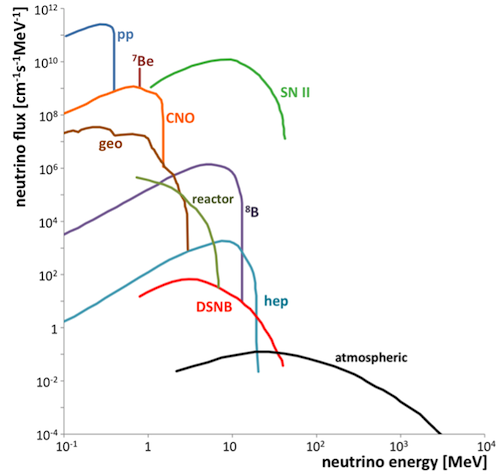
\includegraphics[width=\textwidth]{graphics/neutrinos/neutrinoSpectrum.png}
		\end{minipage}
		\begin{minipage}{0.34\textwidth}
		\caption[Neutrino Sources]{~}A graph summarizing different neutrino sources fluxes both natural and artificial. The sun is the most prominent neutrino source, contributing through various nuclear fusion chains (pp, 7Be, CNO, 8B, hep). The energy range between 1 and 100 MeV is dominated by supernovae type II. Further natural sources are geoneutrinos in the energy regime up to a few MeV, the diffuse supernovae background between 1 and 100 MeV and atmospheric neutrinos beyond 1 MeV. The only artificial source are nuclear reactors, producing neutrinos of energies between 1 and 10 MeV. Figure from \cite{fraenkle}.
		\label{fig:neutrinos:neutrinoSources}	
		\end{minipage}
% 		\begin{figure}
% 		\centering
% 			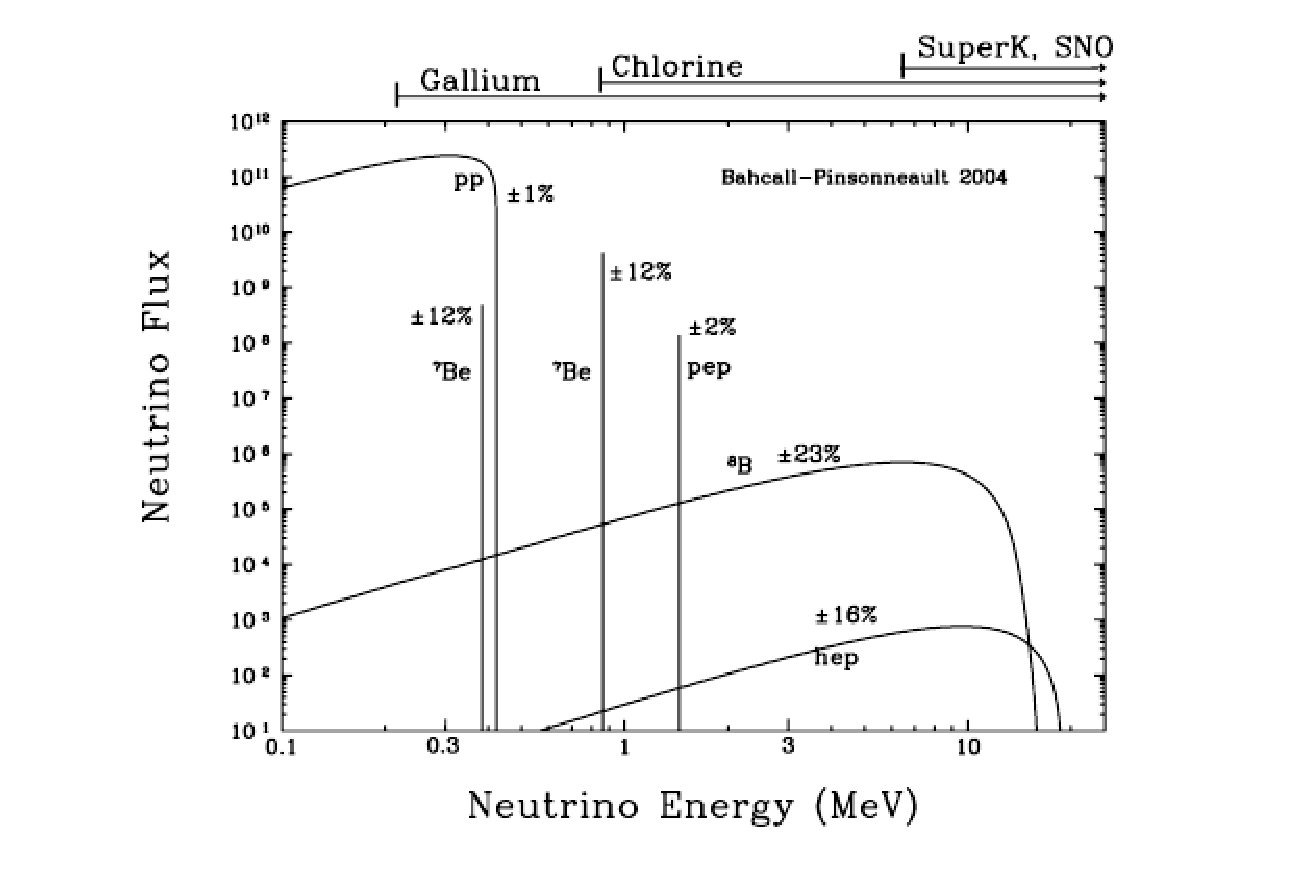
\includegraphics[width=0.8\textwidth]{graphics/neutrinos/solarNeutrinos.eps}
% 			\caption[Solar neutrino Flux]{The graph shows the theoretical solar neutrino flux in \SI{}{\per\square\centi\meter \per\second \per\mega\electronvolt} over the neutrino energy - for line sources in \SI{}{\per\square\centi\meter \per\second}. Different processes are shown, the dominant pp process is visible in the upper left. CNO fluxes are dropped in this figure. On the very top, the sensitivities of different experiments are shown.}
% 			\label{fig:neutrinos:solarNeutrinos}
% 		\end{figure}
		
	\end{figure}
	\begin{itemize}
	\item {\bf Primordial neutrinos}\\
		Lingering around since the ``Big Bang'', neutrinos with thermal energies at $T_\nu\approx \SI{1.95}{\kelvin}$ form a cosmic neutrino background. These neutrinos decoupled shortly after the Big Bang when the weak interaction rate dropped below the expansion rate of the Universe. Due to this "freeze-out" of thermal equilibrium with the other particles, mainly protons, neutrons, and electrons, a relic neutrino density of 336~cm$^{-3}$ is found nowadays.
	\item {\bf Supernovae neutrinos}\\
		Supernovae type II, which occur less often than the type I and only in stars with $M> 8M_\odot$, are known to produce large quantities of neutrinos. Inside the burned-out collapsing star, the electrons' degeneracy pressure leads to de-leptonization of the core by electron capture:
		\begin{equation}
			\ce{e- + p -> n + \nu_e}.
		\end{equation}
		This process produces high energy neutrinos, which can leave the core and carry away energy in the process - and large quantities of that. About \SI{99}{\percent} of the energy released during a type II supernova cooling phase is carried away by neutrinos.

	\item {\bf Solar neutrinos}\\
		The dominant energy production mechanism is the pp reaction chain \ref{ppChain}, which produces neutrinos in a continuous energy range up to a maximum of 0.42 MeV. Additional subdominant fusion chains release neutrinos of higher energies:
		\begin{align}
		\label{ppChain}
			\ce{^1H + ^1 H} & \ce{ -> ^2 He + e+ + \nu_e} && (\SI{0.42}{\mega\electronvolt})\\
			\ce{^8B } & \ce{-> ^8Be + e+ + \nu_e} && (\SI{14.06}{\mega\electronvolt})\\
			\ce{^3He + p } & \ce{ -> ^4He + e+ + \nu_e} && (\SI{18.77}{\mega\electronvolt})
		\end{align}

		Further on, electron capture processes add line spectra to the picture
		\begin{align}
			\label{eq:Berillium}
			\ce{^7Be + e-} & \ce{-> ^7Li + \nu_e}\\
			\ce{^1H + ^1H + e-} & \ce{-> ^2He + \nu_e} (\SI{1.55}{\mega\electronvolt})
		\end{align}
		where $^7$Be emits at two energies: mostly at \SI{0.86}{\mega\electronvolt} (\SI{90}{\percent}) and another, lower energy line at \SI{0.38}{\mega\electronvolt} (\SI{10}{\percent}) \cite{bethgeKernphysik}.\\
		These reactions are responsible for the largest part of the solar neutrino flux through the earth. Predictions on this flux are shown in figure \ref{fig:neutrinos:neutrinoSources} together with other model calculations on flux expectations.
		Solar neutrinos were essential for oscillation research thereby proving that neutrinos are in fact massive (see chapter \ref{ch:Introduction:sec:neutrino Oscillations}).


	\item {\bf Atmospheric neutrinos}\\
		As described in section \ref{ch:Introduction:sec:Cosmic Air Showers} cosmic rays, consisting mostly of protons, constantly impact onto the upper layers of the atmosphere. There, they create air showers, cascades of the initial high energy particles into thousands of particles of lower energies. In that process, muons are created which can significantly contribute to the background of KATRIN.
	\item {\bf Reactor neutrinos}\\
		Nuclear fission produces large quantities of neutrons that decay according to
		\begin{equation}
			\ce{n -> p + e- + \bar\nu_e}
		\end{equation}

		A fission reactor, in which many of these reactions concur, is hence a strong source of neutrinos, depending on the reactor's size. On average, around 6 neutrinos per fission reaction emerge. These sources are used in many experiments, among other things to prove the existence of neutrino oscillations (see chapter \ref{ch:Introduction:sec:neutrino Oscillations}). The Daya Bay experiment for example was able to attest the disapperance of $\bar\nu_e$ , thereby determining the last mixing angle $\theta_{13}$ \cite{dayaBay}.
	\item {\bf Neutrinos from $\beta$ decays}\\
		Very important for the KATRIN experiment are neutrinos from beta decays, more precisely the tritium beta decay. This is described in more detail in chapter \ref{ch:The KATRIN experiment:sec:Measurement Principle}.
	\end{itemize}

	
	
    \section{Neutrinos in the standard model}
    \label{ch:Introduction:sec:Neutrinos in the Standard Model}
    In the second half of the 20th century, the Standard Model was developed, which describes nowaday's particle physics most precisely. It contains six quarks and six leptons, each group divided into three particle generations. making up the matter as well as four types of gauge bosons. The latter are carriers of interactions via the exchange between the Standard Model particles.
    Lately, proof for existence of the Higgs particle, a scalar boson, responsible for the generation of particle masses, was found at CERN \cite{CMS, ATLAS}. It was the last missing piece to complete the Standard Model.
    For our universe, gravity, mediated by the graviton, plays a major role for formation and stability of the larger structures. In particle physics investigations however, it can mostly be neglected. Here, only the strong and weak as well as the electromagnetic interaction contribute noticeably to phenomena observed. That is why, in the standard model, gravity as well as its carrier, the graviton, are disregarded.
    \begin{figure}
    	\centering
    	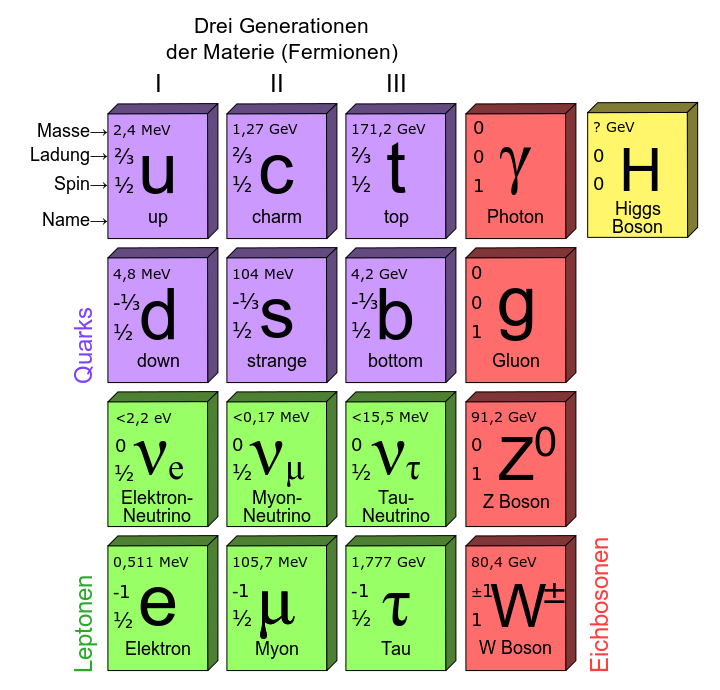
\includegraphics[width = 0.6\textwidth]{graphics/standardModel/Standard_Model_of_Elementary_Particles-de.png}
    	\caption[Standard Model Particles]{Particle content of the standard model. Upper left, purple: Quarks, the building blocks of hadrons. Lower left, green: Leptons, which neutrinos belong to. Right, red: Bosonic force carriers. Upper right, yellow: Higgs particle. \cite{particlesSM}}
    	\label{fig:standardModel:particles}
    \end{figure}
	
    Most of what we can experience in our daily life or in experiments at low energies is attributable to the electromagnetic force or gravity, however, strong and weak interaction do play a major role when it comes to high energy physics, where their limited reach is overcome by small distances between interacting particles. In case of the neutrino, its detection and thereby study of its characteristics is very difficult as it interacts only gravitationally and weakly. Although the weak interaction is a lot stronger compared to gravity, it is still weak compared to both electromagnetic and strong interactions\ref{tab:interactionStrengths}. Therefore the neutrino is considered elusive, the detection efficiencies are low and only large scale detectors are able to
	detect statistically relevant amounts of neutrinos.
    \begin{table}
    \centering
        	\caption[Elementary Interactions]{A comparison of the strength of the different interactions relative to the strong force and of their ranges \cite{povh}.}
		\label{tab:interactionStrengths}
    	\begin{tabular}{|l|cccc|}
    		\hline
    		Force & strong & electromagnetic & weak & gravitation\\
    		\hline
    		\rule{0pt}{3ex} relative strength & 1 & \SI{e-2}{} & \SI{e-5}{} & \SI{e-40}{}\\
    		range & $\approx\SI{1}{\femto\meter}$ & $\infty$ & $\approx\SI{e-3}{\femto\meter}$ & $\infty$\\
    		\hline
    	\end{tabular}

    \end{table}

    One method used quite frequently is the Cherenkov radiation emitted by particles traveling through matter faster than the matter-specific speed of light. The occurring cones of light, comparable to the supersonic cones caused by planes in air, can be detected by photomultiplier tubes. The challenges are the large target volumes and a maximization of the surface coverage with PMTs, which are required to determine the direction and energy of the incoming neutrino. This is why most experiments make use of ``natural'' detectors such as water, e.g. Super-Kamiokande and Antares, \cite{Antares, PhysRevLett.110.181802} or ice \cite{iceCube}.
    Other approaches rely on the inverse beta decay of reactor neutrinos within the target material:
    \begin{equation}
		\ce{\bar\nu_e + p -> e^+ + n}.
    \end{equation}
   
    
   
    
    \section{Neutrino Oscillations}
    \label{ch:Introduction:sec:neutrino Oscillations}
     In the Standard Model, neutrinos are considered to be massless. 
    Many experiments such as Kamiokande \cite{PhysRevLett.110.181802}, Daya Bay \cite{dayaBay2} or SNO \cite{SNOOscillations} though have shown that neutrinos are indeed massive by observation of neutrino oscillations with both reactor neutrinos and solar neutrinos.
    Important for those experiments is the precise knowledge of the source distance to detector and the energy distribution of the neutrinos.
    
    However, until now, only the mixing angles and the differences of the squared masses are known. While the mixing angles determine the flavor content of each mass eigenstate, see figure \ref{fig:massSchemes}, the absolute mass scale is fixed by the lightest mass eigenstate $m_{\text{min}}$, which is not known, see figure \ref{fig:massHierarchy}. Two mass schemes are possible: the normal and the inverted one. Normal means that the smallest number also describes the smallest mass state, i.e. $m_{\nu_1} < m_{\nu_2} < m_{\nu_3}$. In the inverted scheme, the squared mass difference of eigenstates two and three is not directed upwards, but pushes the $m_{\nu_3}$ mass below the other two.
    
    \begin{figure}
    \centering
    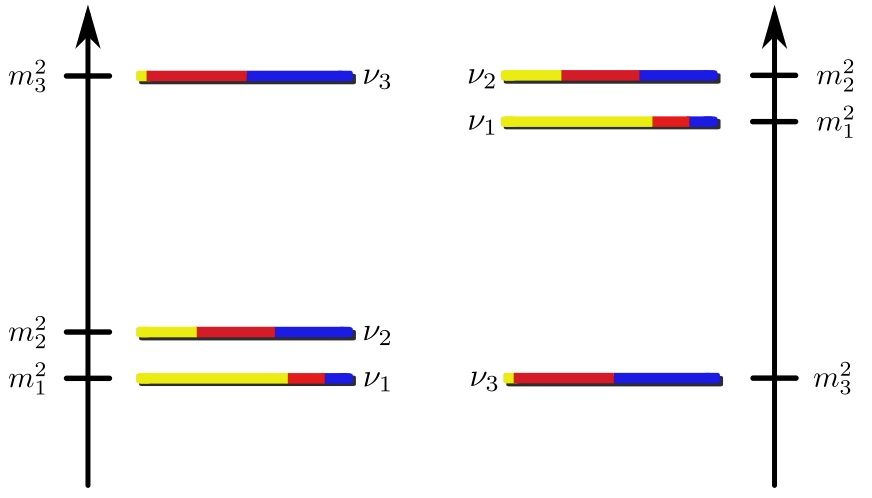
\includegraphics[width=0.7\textwidth]{graphics/standardModel/massHierarchy.jpg}
    	 \caption[Neutrino Mass Hierarchy]{The possible mass hierarchies for neutrinos. Left: normal scheme with $m_{\nu_1} < m_{\nu_2} < m_{\nu_3}$. Right: inverted scheme where $m_{\nu_1} < m_{\nu_2}$ is still true, though $m_{\nu_3} < m_{\nu_1}$. The colored bars represent the corresponding flavor content, i.e. the probability of measuring a specific flavor eigenstate when detecting a pure mass eigenstate. Yellow represents$\nu_e$, red $\nu_\mu$ and blue $\nu_\tau$ \cite{neutrinoMassScheme}.}
    	\label{fig:massSchemes}
    \end{figure}
    \begin{figure}
    \centering
    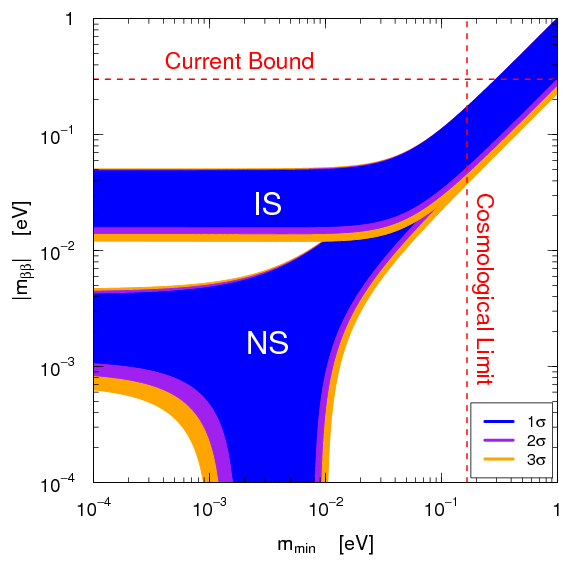
\includegraphics[width = 0.7 \textwidth]{graphics/standardModel/massSchemes.png}
	\caption[Effective Neutrino Mass]{The possible effective masses for neutrinos depending on the lightest neutrino mass $m_{min}$ shown on the x-axis. Normal and inverted scheme are marked NS and IS. The current bound from $0\nu\beta\beta$ decay is displayed as well as cosmological limitations. }
    	\label{fig:massHierarchy}
    \end{figure}

    
      If the neutrinos were massless, their mass eigenstates would equal their flavor eigenstates.
    First hints against this assumption occurred as inconsistencies between the measured and the calculated solar $\nu$-flux occurred in experiments at the Homestake mines \cite{homestake}. To explain the missing $\nu_{e}$, the theory of neutrino oscillations emerged, where each flavor is made up of all three mass eigenstates. This mixture is described by the so called Pontecorvo-Maki-Nakagawa-Sakata matrix:
        \begin{equation}
        \left(
        \begin{array}{c}
	 \left |\nu_e\right>\\
	 \left |\nu_\mu\right>\\
	 \left |\nu_\tau\right>\\
        \end{array}
        \right)
	 = \left(
	\begin{array}{ccc}
      	U^*_{e,1} & U^*_{e,2} & U^*_{e,3}\\
      	U^*_{\mu,1} & U^*_{\mu,2} & U^*_{\mu,3}\\
      	U^*_{\tau,1} & U^*_{\tau,2} & U^*_{\tau,3}\\
      	\end{array}
	\right)
	\left(
	\begin{array}{c}
      	\left|\nu_1\right>\\
      	\left|\nu_2\right>\\
      	\left|\nu_3\right>\\
    	 \end{array}
    	 \right)
    \end{equation}
    In this equation, the matrix U can be parametrized through a combination of three rotation matrices and a complex phase factor $\delta_D$, the so called Dirac phase, as well as two complex Majorana phases $\delta_M$
    
    \begin{equation}
	\centering
	\begin{split}
     U = \left(
	\begin{array}{ccc}
      	1 & 0 & 0\\
      	0 & c_{23} & s_{23}\\
      	0 & -s_{23} & c_{23}\\
   	\end{array}
	\right)
	\left(
	\begin{array}{ccc}
      	c_{13} & 0 & s_{13}e^{-i\delta_D}\\
      	0 & 1 & 0\\
      	-s_{13}e^{-i\delta_D} & 0 & c_{13}\\
      	\end{array}
	\right)\cdot\\
	\cdot\left(
	\begin{array}{ccc}
      	c_{12} & s_{12} & 0\\
      	-s_{12} & c_{12} & 0\\
      	0 & 0 & 1\\
      	\end{array}
	\right)
		\left(
	\begin{array}{ccc}
      	e^{i\delta_{M1}} & 0 & 0\\
      	0 & e^{i\delta_{M2}} & 0\\
      	0 & 0 & 1\\
      	\end{array}
	\right)
	\end{split}
    \end{equation}
    where $c_{ij}=\cos{\theta_{ij}}$ and $s_{ij}=\sin{\theta_{ij}}$.\\
	Initially, the neutrino is created in a pure flavor eigenstate $\nu_{\alpha}$, which can be described by the three matrix elements and the corresponding mass eigenstates:
	\begin{equation}
		\left|\nu_\alpha(t=0)\right> = U^*_{\alpha1} \left|\nu_1\right> + U^*_{\alpha2} \left|\nu_2\right> + U^*_{\alpha3} \left|\nu_3\right>.
	\end{equation}
	The time evolution of this state now reveals the oscillatory behavior of the neutrino, as evolving states are no longer pure flavor eigenstates:
	\begin{equation}
		\left|\nu_\alpha(t>0)\right> = U^*_{\alpha1} e^{-iE_{\alpha1}t}\left|\nu_1\right> + U^*_{\alpha2} e^{-iE_{\alpha2}t}\left|\nu_2\right> + U^*_{\alpha3}e^{-iE_{\alpha3}t} \left|\nu_3\right> \neq \left|\nu_\alpha\right>.
	\end{equation}
	The time-dependent probability to find a certain flavor eigenstate $\left|\nu_{\alpha}\right>$ is then given by
	\begin{equation}
		\begin{split}
			\left|\nu_\alpha(t)\right> = \sum_{k = 1,2,3} U^*_{\alpha k}\exp\left(-iE_k t\right)\left|\nu_k\right>.
		\end{split}
	\end{equation}
	If the mass eigenstates in turn are expressed as a mixture of flavor eigenstates, one can extract the prefactor of the sum's components as the transition probability for each single flavor:
	\begin{equation}
		P(\nu_\alpha \rightarrow\nu_\beta) = \left| \left<\nu_\beta\right|\left.\nu_\alpha(t)\right>\right|= \left|\sum_{k=1,2,3}U^*_{\alpha k} \exp{\left(-iE_kt\right)}U_{\beta k}\right|^2
	\end{equation}
	Table \ref{tab:neutrinoParameters} summarizes the experimental results for the mixing angles and squared mass differences.
	\begin{table}
	\centering
		\caption[Neutrino Parameters]{Given are the latest measurement results of the mixing angles and squared mass differences. For $\sin^2{\left(2\Theta_{23}\right)}$, only the lower limit is given \cite{reviewOfParticlePhysics}.}
		\label{tab:neutrinoParameters}
		\begin{tabular}{|c|c|}
		\hline
			parameter & value\\
			\hline			
			$\sin^2{\left(2\Theta_{12}\right)}$& \SI{0.875\pm 0.024}{}\\
			$\Delta {m^2}_{21}$&\SI{7.5 \pm 0.20 e -5}{\square\electronvolt}\\
			$\sin^2{\left(2\Theta_{23}\right)}$& >\SI{0.95}{}\\
			$\Delta {m^2}_{32}$ & \SI{2.32(12)}{\square\electronvolt} \\
			$\sin^2{\left(2\Theta_{13}\right)}$ & \SI{0.095\pm0.010}{}\\
			\hline
		\end{tabular}
		
	\end{table}
	Though the mixing angles and mass differences have been determined, more precise measurements are required to determine the mass hierarchy and the CP-violating phase(s). For this purpose, new experiments such as LENA \cite{LENA} are being built.
	
	    \section{Indirect measurement of the neutrino mass}
    \label{ch:Introduction:sec:Massive neutrino:subsec:indirect Neutrino Mass measurement}
   	The absolute neutrino mass scale can be accessed indirectly, through data that is affected by a non-zero neutrino mass but where this mass itself is not a direct observable. The main approaches, namely the neutrinoless double beta-decay and cosmological observations, are shortly discussed in the following.\\\\
   	\paragraph{Neutrinoless double beta decay ($0\nu\beta\beta$)}
   	The double beta decay process ($2\nu\beta\beta$) in which two neutrinos are emitted, only occurs if the single $\beta$ decay to the $^A_{Z+1}X$ daughter nucleus is prohibited by energy conservation. Within the 2$\nu\beta\beta$ decay
   	\begin{equation}
   		\ce{^A_ZX -> ^A_{Z+2}X + 2 e- + 2 \bar\nu_e}.
   	\end{equation}
   	two neutrinos are emitted alongside two electrons. In contrast, no neutrinos are emitted within the 0$\nu\beta\beta$ decay, which can exist only if the neutrino is its own anti-particle, a so called Majorana neutrino. Then, if a nucleus undergoes double beta decay, the neutrino from one vertex can be absorbed in the second vertex as an anti-neutrino with inversed helicity - or vice versa. As this change in helicity is only possible for a massive particle, the $0\nu\beta\beta$ decay would be further proof of a massive neutrino. Furthermore, as the probability for a helicity change depends on the particle mass, the decay rate, and consequently the half life $t_{1/2}$, depend on the effective Majorana neutrino mass \cite{currentNeutrinoSearches}:
    \begin{equation}
    	\Gamma_{0\nu\beta\beta} \propto \left| \sum^3_{i-1}{U_{ei}^2m\left(\nu_i\right)}\right|^2.
    \end{equation}
    
    \paragraph{Cosmological observations}
    The problem can also be approached by calculations using astrophysical data.\\
    For one, the formation of structures in the universe depends on the neutrino mass. Acting as hot dark matter, neutrinos wash out small scale structures. Consequently, small scale fluctuations in the matter power spectrum are suppressed by massive neutrinos. Using the spectroscopic data from galaxy surveys like SDSS \cite{SDSS} or studying the cosmic microwave background like WMAP \cite{WMAP} or Planck \cite{Planck}, an upper limit of $\sum_\nu m_\nu < \SI{0.6}{\electronvolt}$ can be obtained.\\
	As these indirect methods for neutrino mass measurements strongly depend on model assumptions, the direct methods, which are discussed in the next section, play a key role in the determination of a model-independent value of the neutrino mass.

    
    \section{Direct measurement of the neutrino mass}
    \label{ch:Introduction:sec:Massive neutrino:subsec:direct Neutrino Mass measurement}
    Direct measurements of the neutrino mass rely on a precise determination of the electron energy spectrum of single $\beta$ decay. The advantage of direct measurements is that they only rely on the relativistic energy-momentum-relation $E^2 = m^2c^4 + p^2c^2$., which makes the results mostly model independent. There are spectrometric as well as calorimetric approaches. To increase their sensitivity, current experiments have to be scaled up either in size (spectrometer) or in target mass (calorimeter). With the KATRIN experiment, the spectrometer approach has reached its technical limits. Although the calorimetric approach is further scalable, the necessity of ten thousands of single detectors is a big challenge. A big advantage of the KATRIN experiment is the ability to select only the spectral part close to the decay endpoint, which is relevant for the neutrino mass determination. Consequently, a high luminosity can be achieved without suffering from pile-up effects.
    Tritium was chosen as $\beta$-emitter for several reasons listed below.
    \begin{itemize}
    	\item A high luminosity is ensured by the short half life of $t_{1/2} = \SI{12.3}{\year}$. Consequently, small amounts of the emitter are sufficient to ensure good statistical results.
    	\item At the same time, the inverse of the cubic endpoint energy ($1/E_0^3$) defines the amount of electrons emitted in the endpoint region (up to \SI {1}{\electronvolt} below the endpoint). Tritium's low endpoint energy of \SI{18.6}{\kilo\electronvolt}, undercut only by one $\beta$ emitter, rhenium, that has other disadvantages, ensures a high luminosity at the detector.
    	\item As tritium beta decay is a superallowed process \cite{superallowance}, the matrix element $\left|M_{had}\right|$ is energy independent, which significantly simplifies the analysis procedures.
    	\item Another simplification compared to other $\beta$-emitters is the easily calculable electron shell configuration, which allows a determination of the spectrum of excited states.
    	\item Concerning scattering of signal electrons on tritium atoms in the source volume, the low atomic number makes for small cross sections in inelastic scattering. This reduces energy smearing inside the source volume.
    \end{itemize}
    These reasons make tritium the element of choice for KATRIN.\\\\
    The above mentioned rhenium is used in the calorimetric approach. Experiments like MARE \cite{MARE2007} use rhenium in bolometers as both emitter and detector. The low endpoint energy of \SI{2.47}{\kilo\electronvolt} results in a large fraction of electrons with energies near this endpoint. However, this is largely compensated by the much longer half life of $t_{1/2} = $\SI{4.32 e 10}{\year}. Still, the mass of rhenium required to gain statistically relevant results remains below the tritium mass used in KATRIN. The MARE strategy is to split the radioactive material and use it in many small micro-bolometers. That is beneficial as readout is slow and the rate per bolometer is reduced by lowering the emitter mass. Thermistors then sample the temperature, catching peaks induced by electrons from $\beta$ decays scattering inside the solid source.
    The experiment set up by the Milano collaboration has set an upper limit of
    \begin{equation}
    	m_{\bar\nu_e} < \SI{15}{\electronvolt} ~ {\rm at}~ \SI{90}{\percent\CL}.
    \end{equation}
    This limit shall be pushed to \SI{0.2}{\electronvolt} according to \cite{MARE2007}.  

	\section{Cosmic rays from the viewpoint of KATRIN}
    \label{ch:Introduction:sec:Cosmic Air Showers}
    When high energy particles hit the upper atmosphere, a cascade of particles, generated from the interaction with atmospheric molecules and atoms, follows. Most primary particles are nucleons, most of which again are free protons (85\%), i.e. hydrogen ions, followed by $\alpha$ particles (15\%). The flux of helium nuclei is already about an order of magnitude below the hydrogen ones and higher mass number nuclei show even lower rates, see figure \ref{fig:Introduction:sec:CosmicRays} \cite{highEnergyCosmicRays}.
    \begin{figure}
	\begin{minipage}[d]{0.49 \textwidth}
		  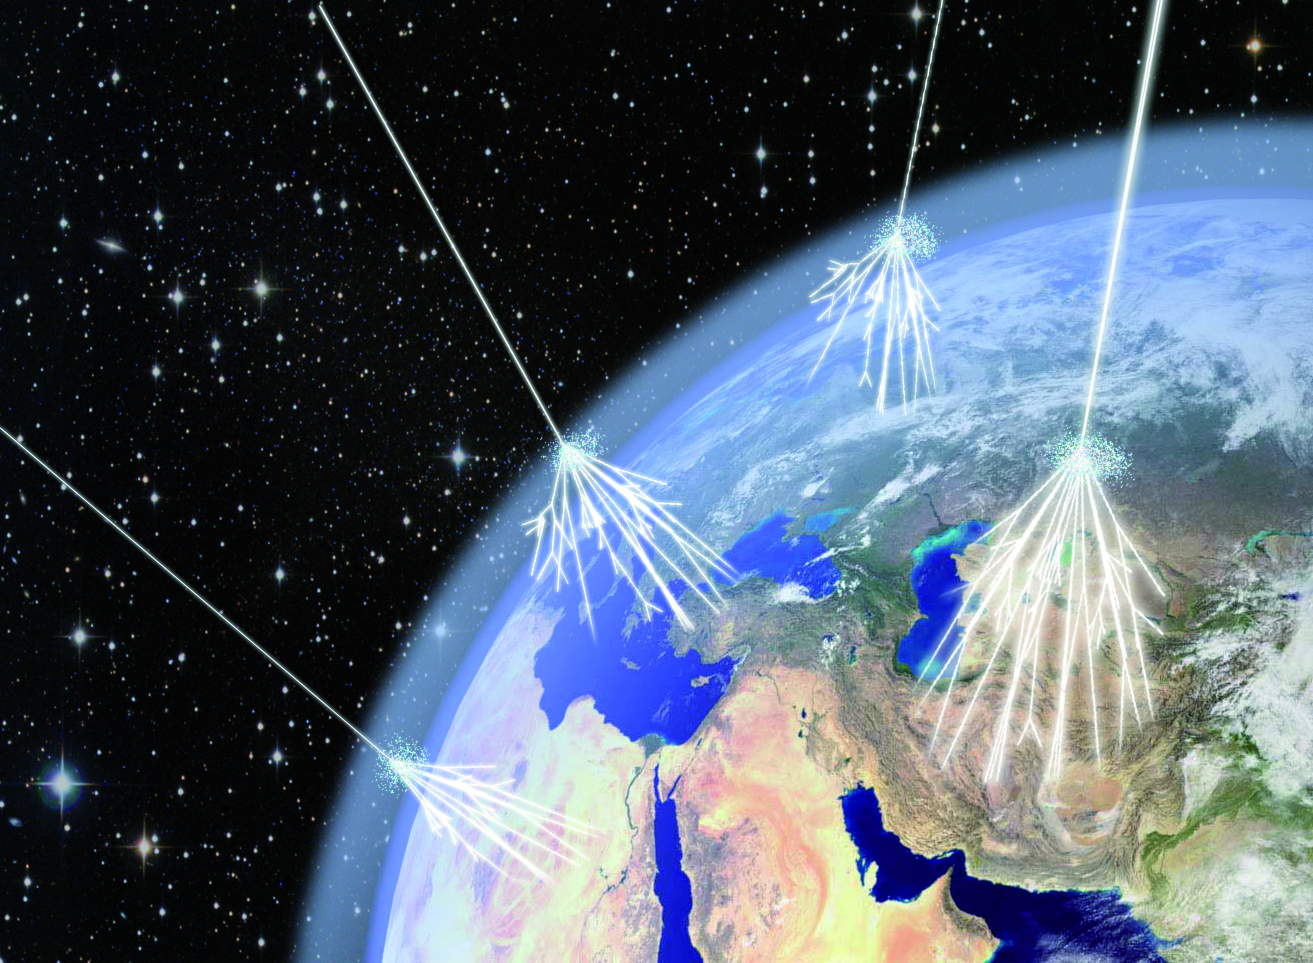
\includegraphics[width=\textwidth]{graphics/cosmicRays/cosmicRays.jpg}
	\end{minipage}
	\begin{minipage}[d]{0.49 \textwidth}
		  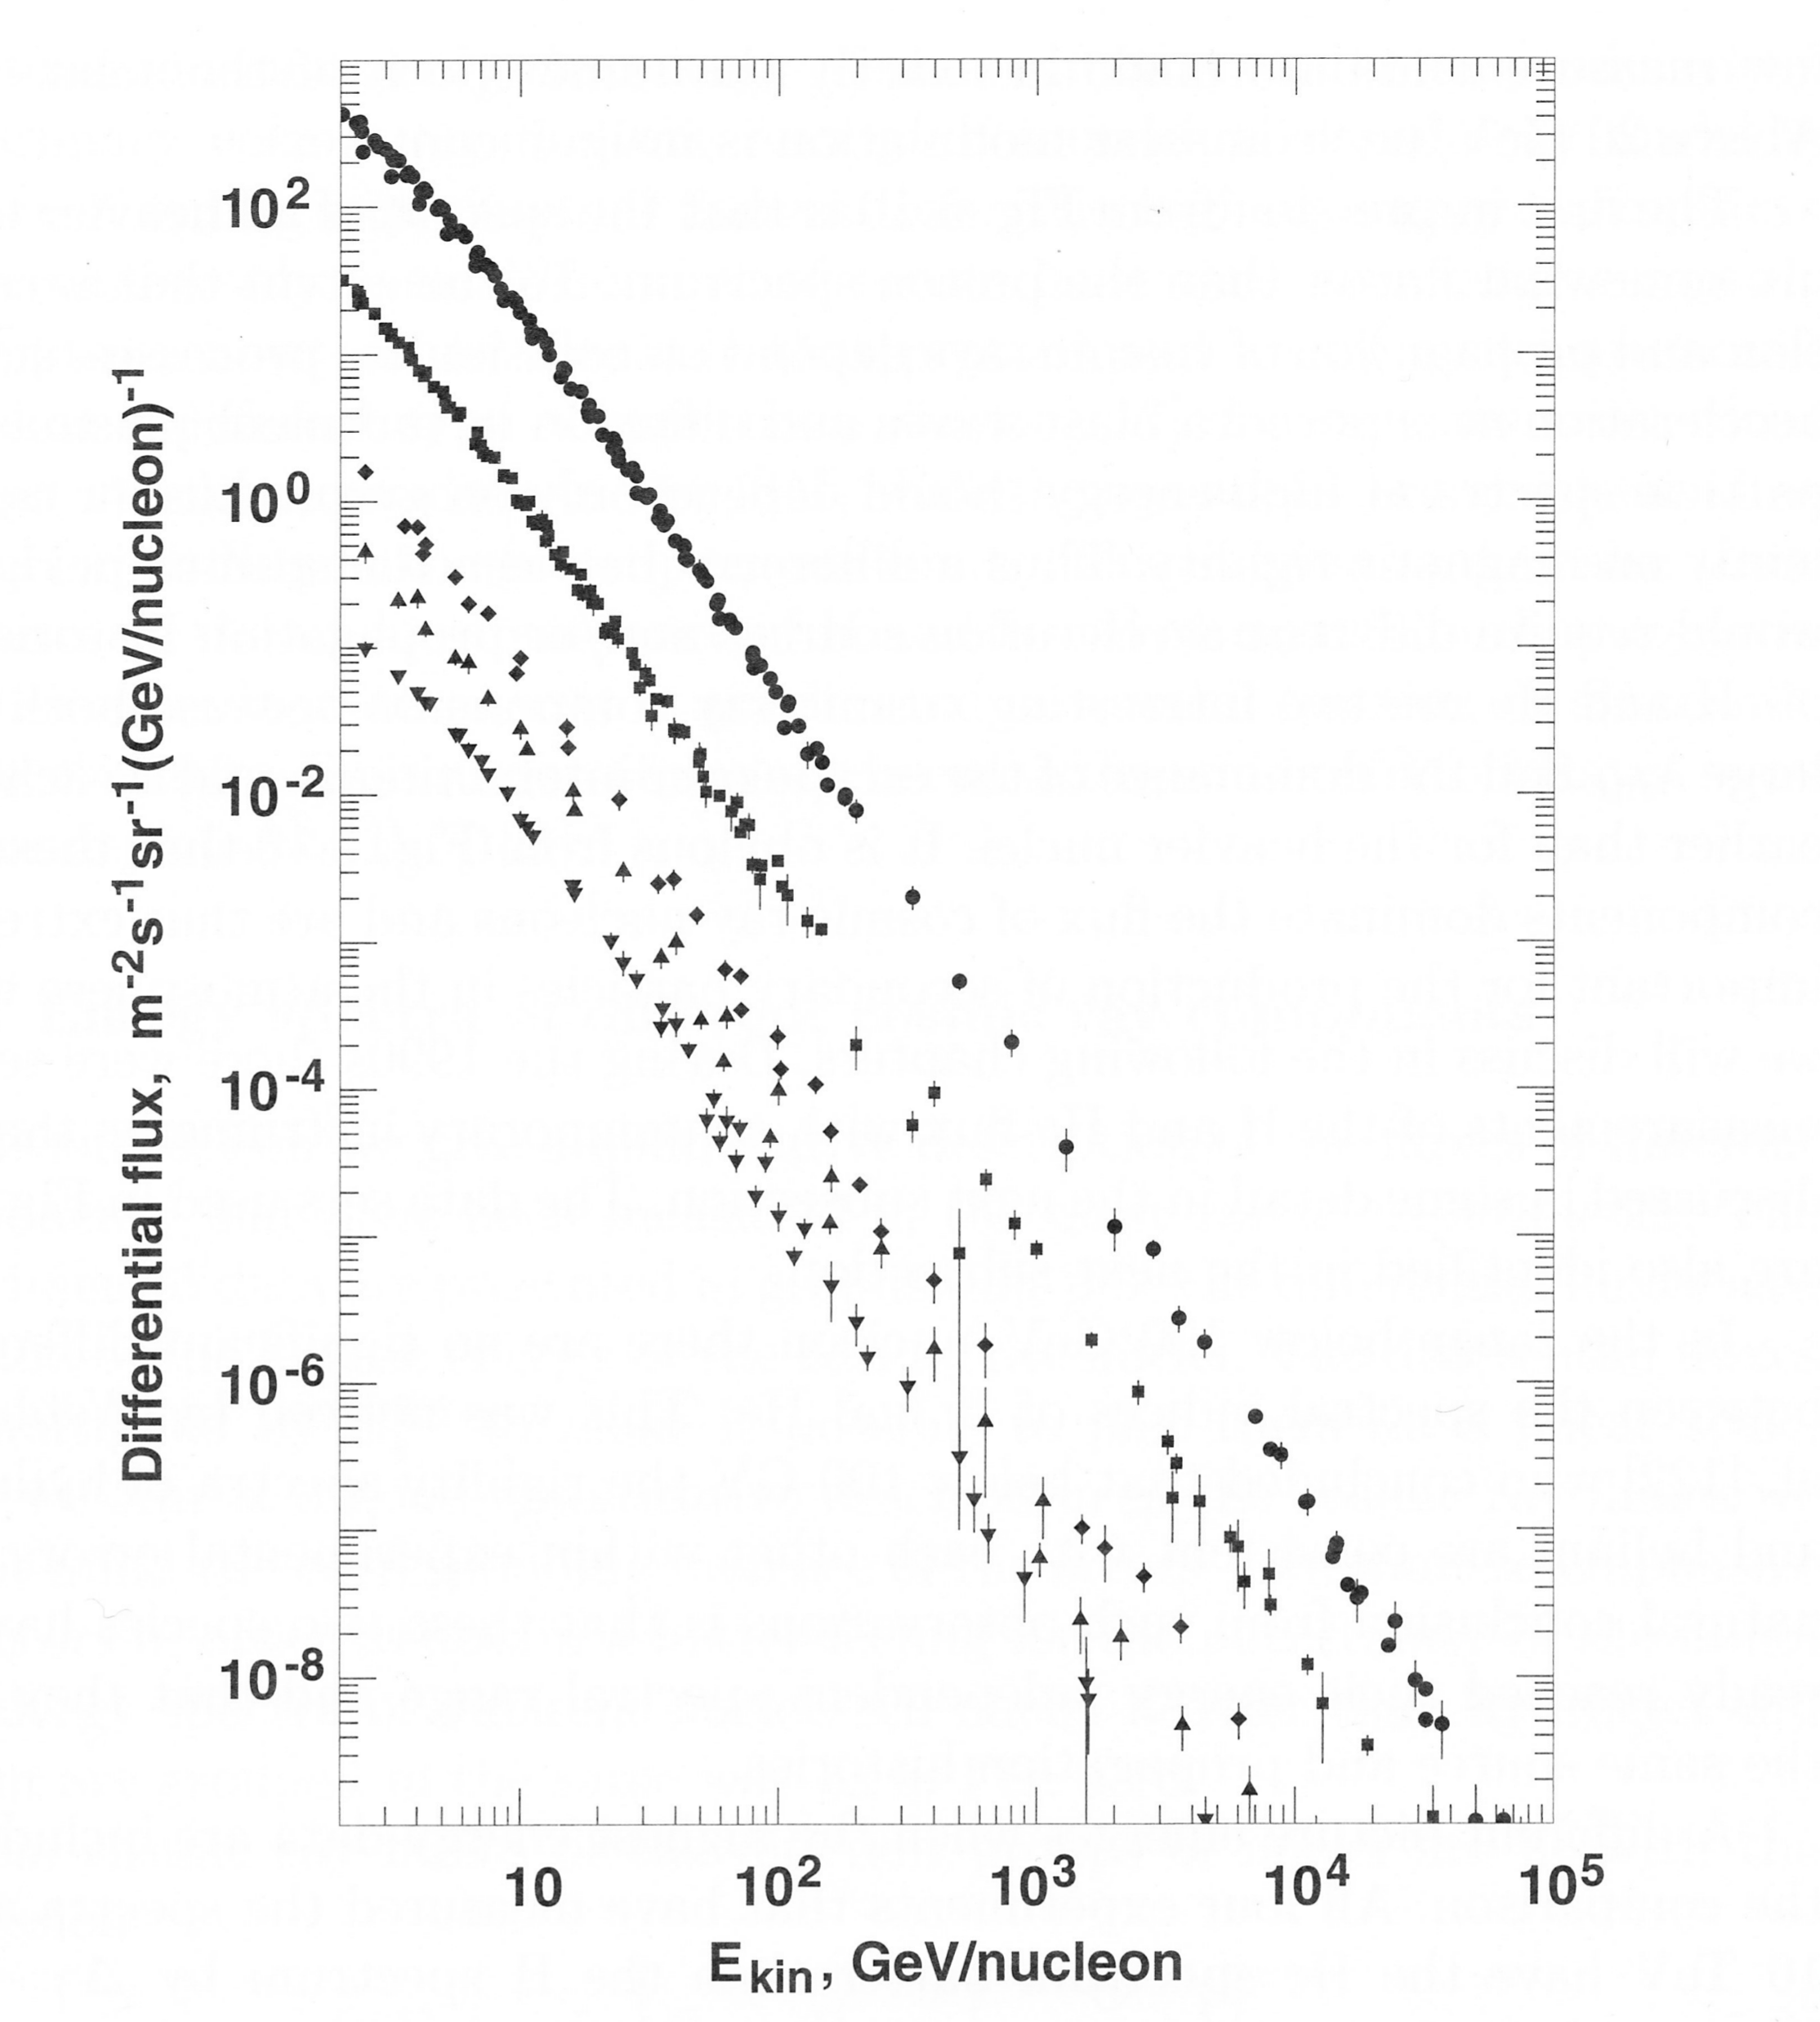
\includegraphics[width=\textwidth]{graphics/cosmicRays/energySpectrum.png}
	\end{minipage}
	\caption[Cosmic Ray Composition]{Left, an artistic impression of various cosmic rays hitting the atmosphere \cite{airShower}. Right, the measured composition for cosmic nuclei is shown: The lightest particle, the proton exhibits the largest flux, while heavier ions are suppressed by several orders of magnitude. Figure from \cite{highEnergyCosmicRays}.}
	\label{fig:Introduction:sec:CosmicRays}
    \end{figure}
    A large number of secondary particles is created via electromagnetic, inelastic hadronic and nuclear interactions, which are detailed in the following \cite{highEnergyCosmicRays, Grupen}. 
    \begin{itemize}
    	\item {\bf Nuclear fragmentation}\\
    	For very high energy primary particles above the separation energy $E_s$ according to 
		\begin{equation}
			E_s \simeq E_b(N,Z) - E_b(N_F, Z_F) - E_b(N - N_F, N - Z_F) - \frac{Z_F(Z -Z_F)}{(A-F)^{1/3}}
		\end{equation}
		it is possible to fragment a nucleus. The first three terms describe the binding energies of the nuclei involved, the last term accounts for the Coulomb barrier. Especially for high-Z nuclei, more effects become relevant and one has to rely on empirical descriptions of the problem.
		\item{\bf Inelastic hadronic interaction}\\
		For high energies, quantum chromo dynamics describe the interactions of particles sufficiently well, while for energies below \SI{1}{\TeV} one has to rely on phenomenological descriptions. These interactions are prominent in the production of secondary particles like pions or kaons.
		
		\item{\bf Electromagnetic interaction}\\
		The electromagnetic component is the main interaction channel for lighter, charged particles like muons or electrons, but also for photons. As the propagation of muons is especially important in the context of this thesis, these interactions will be described in some more detail.
	
	
	\begin{itemize}
		\item {\bf Coulomb scattering}\\
		If one charged particle passes another, it is deflected by its electric field by the angle $\theta$ according to
		\begin{equation}
			\tan{\frac{\theta}{2}} = \frac{zZe^2}{Mv^2b}
		\end{equation}
		where $z$ and $Z$ are the charge numbers of scatterer and scattering particle, $e$ is the elementary charge, $M$ the reduced mass and $b$ the impact parameter.
		\item{\bf Ionization losses}\\
		Through ionization and excitation of molecules, incident particles loose energy in a medium, in this case the atmosphere, according to
		\begin{equation}
			\frac{dE}{dx} = -\frac{N_AZ}{A}\frac{2\pi\left(ze^2\right)^2}{M\nu^2}\left[\ln{\frac{2Mv^2\gamma^2}W{I^2}}-2\beta^2\right],
		\end{equation}
		where $Z$ is the atomic and $A$ the mass number of the medium, and $I$ is the average ionization potential. $N_a$ denotes Avogadro's number, $ze$ the particle charge, $v$ its velocity and $M$ its mass. Furthermore, $\beta = v/c$, $\gamma = 1/\sqrt{1-/\beta^2}$ and $W$ is the maximum energy deposit \cite{Hayakawa}.\\
		This effect is used for muon detection in the KATRIN experiment, see chapter \ref{ch:The muon detection system}.
		
		\item{\bf Compton scattering and inverse compton effect}\\
		Compton scattering is the photonic eqivalent to ionization by charged particles. In the process, a photon interacts with bound electrons and excites or ionizes the corresponding atom. Doing so, the photon looses energy and is shifted towards longer wavelengths.\\
		The inverse Compton effect, as the name suggests, describes a photon gaining energy from an atomic shell electron.
		
		\item{\bf Bremsstrahlung and synchrotron radiation}\\
		When charged particles are deflected by electric fields, photons are emitted and the particle loses energy. The same is applicable to magnetic fields, where the effect is called synchrotron radiation and a time dependent energy loss occurs. The total energy loss for electric fields can be described by
		\begin{equation}
			\frac{dE}{dx} = \frac{4N_AZ^2}{A}\alpha r_e^2 E  \ln{\left(183 Z^{1/3}\right)} = \frac{E}{X_0},
		\end{equation}
		where the radiation length $X_0$ has been introduced to describe the average matter necessary for a particular energy loss.
		
		\item{\bf Electron-positron creation}\\
		A photon of sufficient energy (>\SI{1}{\mega\electronvolt}) can create an electron-positron pair  when scattering at an atomic nucleus. With higher energies, other particles can be created considering the known conservation laws. 
		This proccess can be seen as the inverse bremsstrahlung, assuming the outgoing anti-particle to be its time inverted particle. The energy loss can be described similarly and scales linearly with the energy of the incident particle.

		\item{\bf Cherenkov radiation}\\
		Much smaller amounts of energy are emitted as cherenkov light. The process is particularly important though due to its easily detectable particle indicators. Cherenkov radiation occurs when particles move through matter at speeds above the phase velocity of light $c/n$ for a refractive index $n$. As the atmospheric refractive index is only slightly above 1, particles need to be super-relativistic to emit Cherenkov light. 		
    \end{itemize}
    \end{itemize}
	After cascading mostly through multiple intermediate particles, at sea level about \SI{80}{\percent} of the cosmic particles are muons. These are super-relativistic due to their small masses and, at the same time, high energies. Even at these high speeds, the muons' average decay time of about \SI{2.2}{\micro\second} \cite{muonLifetime} is too small for many muons to reach the earth's surface from our reference frame's point of view. In the average production height of \SI{2}{\kilo\meter} \cite{muonProductionHeight}, the non relativistic time of flight for a particle traveling at 90\% of the speed of light would be 
    \begin{equation}
	t_{class} = \SI{2}{\kilo\meter} / 0.9\cdot c = \SI{7.4}{\micro\second}
    \end{equation}
    The fact that nevertheless, a rather large muon flux is observed at the Earth is explained by time dilation effects of special relativity:
    \begin{equation}
    	t_{rel} = t_{class} / \sqrt{1-0.9^2}
    \end{equation}
    which, from our reference frame, prolongs the muon lifetime by about a factor 5, thereby allowing muons to reach the Earth's surface from heights of \SI{3}{\kilo\meter}. Most muons have even higher energies, enabling them to reach surface from greater heights and with a large angular distribution.
    These muons can cause background events via emission of secondary electrons in the stainless steel vessel of the KATRIN main spectrometer and hence pose a particular challenge. Shielding against muons is difficult as it requires thick layers of dense matter due to the muons high energies and the relatively low energy deposition in matter.
    The fluctuations in the energy deposition of a muon in matter can be described by the Landau distribution that is parametrized as follows \cite{Grupen}:
    \begin{equation}
    	L(E) = \frac{1}{2\pi}\exp{\left\{-\frac{1}{2}\left(E- \hat E + \exp \left(-(E-\hat E)\right)\right)\right\}}.
    \end{equation}
	Here, $\hat E$ is the most probable energy deposition value. The analytic distribution is shown in figure \ref{fig:Introduction:landauDistribution}. It will be shown in section \ref{ch:The muon detection system:sec:Gains, Thresholds and Acceleration Voltages}, that this characteristic distribution can be reproduced by the muon detector system implemented in the course of this thesis.
	\begin{figure}[H]
	\centering
		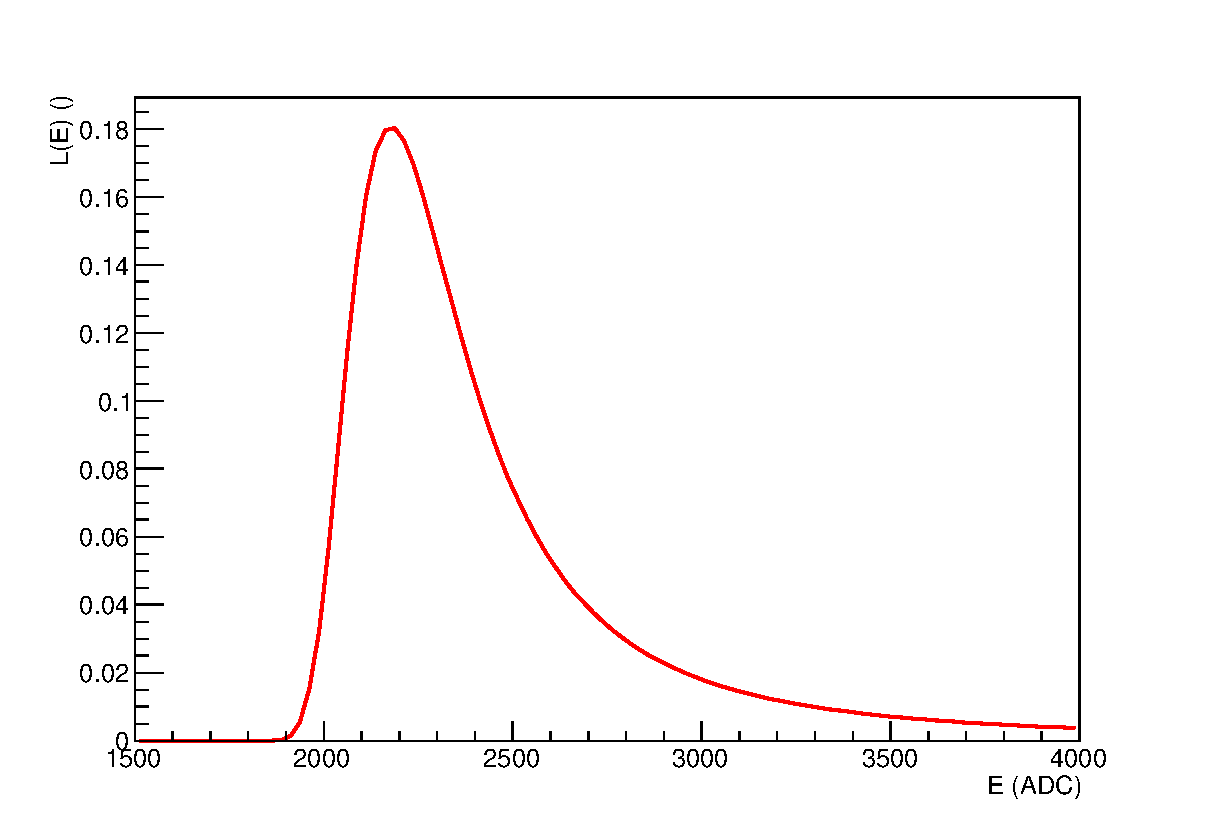
\includegraphics[width = 0.9 \textwidth]{graphics/cosmicRays/TMathLandauRoot.eps}
		\caption[Landau Distribution]{Analyticcal Landau distribution as implemented in the ROOT software. $\hat E$ was set to 1200.}
		\label{fig:Introduction:landauDistribution}
	\end{figure}

    
   